\documentclass[tikz,11pt,border=1cm]{standalone}
%\documentclass[a4paper]{article}

\usepackage{tikz}
\usetikzlibrary{shapes,arrows}

\usepackage{pgfplots}
\pgfplotsset{/pgf/number format/use comma,compat=newest}

\begin{document}

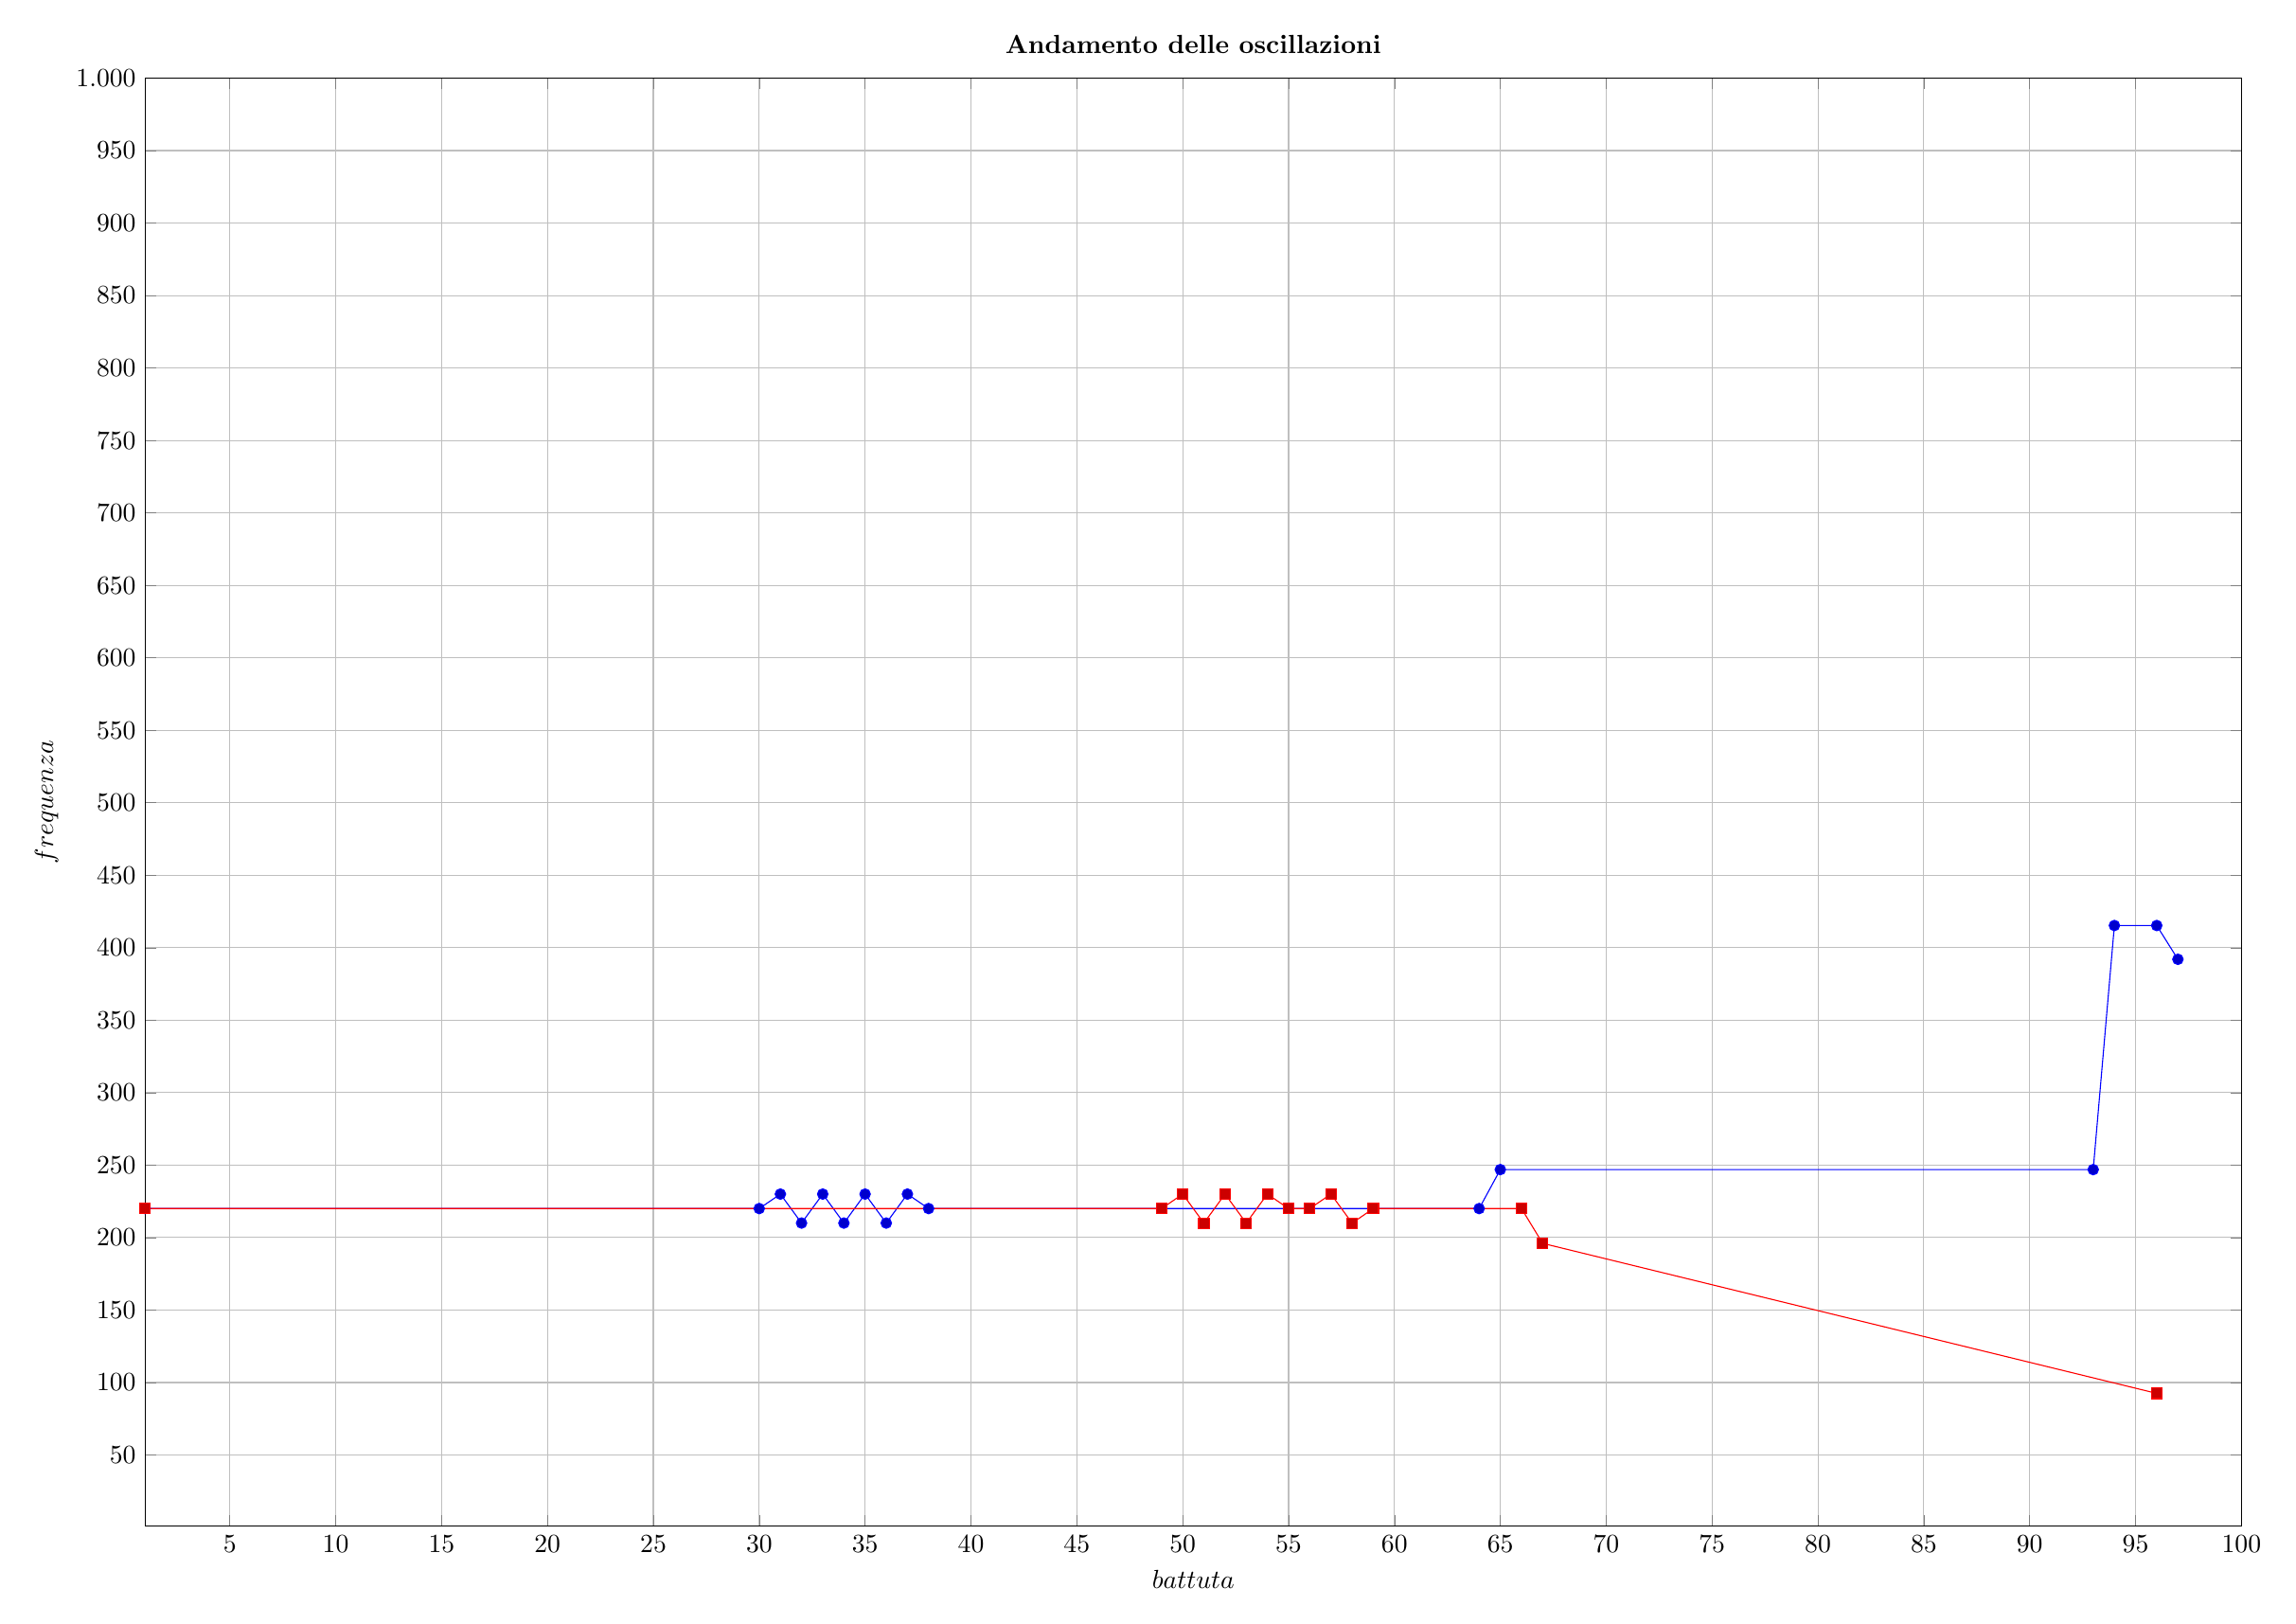
\begin{tikzpicture}
\begin{axis}[xmin=1,
			 xmax=100,
 			 ymin=1,
			 ymax=1000,
			 grid=major,
 			 xlabel=$battuta$,
			 ylabel=$frequenza$,
 			 title={\textbf{Andamento delle oscillazioni}},
 			 width=29.7cm,
			 height=21cm
			 ]
\addplot coordinates
{
(1, 220)
(30, 220)
(31, 230)
(32, 210)
(33, 230)
(34, 210)
(35, 230)
(36, 210)
(37, 230)
(38, 220)
(64, 220)
(65, 246.9)
(93, 246.9)
(94, 415.3)
(96, 415.3)
(97, 392)
};
\addplot coordinates
{
(1, 220)
(49, 220)
(50, 230)
(51, 210)
(52, 230)
(53, 210)
(54, 230)
(55, 220)
(56, 220)
(57, 230)
(58, 210)
(59, 220)
(66, 220)
(67, 196)
(96, 92.5)
};

\end{axis}
\end{tikzpicture}

\end{document}